\raggedbottom

% ---------------------------------------------------------------------------
\section{Derivation and properties}
\label{app:derivation}
% ---------------------------------------------------------------------------

\paragraph{Closed form.} With $G_d=\mathbb{E}_{x\sim\mu_d}[xx^{\!\top}]$, the
objective of Equation~\eqref{eq:obj} is
\begin{equation*}
J(W)=\sum_d w_d\,\tr\!\big[(W-W_d)\,G_d\,(W-W_d)^{\!\top}\big],
\end{equation*}
which is convex and quadratic in $W$, with gradient
$\nabla J=2\sum_d w_d\,(W-W_d)\,G_d$. Setting it to zero gives
\begin{equation*}
W\sum_d w_dG_d=\sum_d w_dW_dG_d .
\end{equation*}
Substituting $W_d=\Wb+\dd_d$, the term $\Wb\sum_dw_dG_d$ appears on both
sides, so $W=\Wb+\dd_\star$ with $\dd_\star\sum_d\Gt_d=\sum_d\dd_d\Gt_d$, which
is Equation~\eqref{eq:solve}. The solution is the same whether one solves for
the weight or for the update.

\paragraph{Shrinkage as a penalty.} Replacing $G_d$ by
$\alpha G_d+(1-\alpha)\,\mathrm{diag}(G_d)$ replaces teacher $d$'s term of $J$
by
\begin{equation*}
\alpha\,\mathbb{E}\big\|(W-W_d)x\big\|_2^2
+(1-\alpha)\sum_i(G_d)_{ii}\,\big\|(W-W_d)_{:,i}\big\|_2^2 .
\end{equation*}
The second term penalizes the deviation of each input column of $W$ from the
teacher's, in proportion to that coordinate's second moment. Since
$\mathrm{diag}(G_d)$ is positive definite whenever every input coordinate is
active, $\sum_d\Gt_d$ is invertible for $\alpha<1$.

\paragraph{Proposition~\ref{prop:conflict}(i): identical statistics give the
average.} If $G_d=G$ for all $d$, write
$\Gt=\alpha G+(1-\alpha)\,\mathrm{diag}(G)$. Then
\begin{equation*}
\dd_\star=\Big(\sum_dw_d\dd_d\Big)\Gt\,\Big(\sum_dw_d\,\Gt\Big)^{-1}
=\frac{\sum_dw_d\dd_d}{\sum_dw_d}.
\end{equation*}
With equal weights this is the mean of the updates, not their sum: \method
reduces to weight averaging, not to task arithmetic, when the teachers cannot
be told apart by their inputs.

\paragraph{Proposition~\ref{prop:conflict}(ii): a dominant teacher is
recovered.} As $w_d/w_e\to0$ for every $d\ne e$, we have
$\sum_d\dd_d\Gt_d\to\dd_e\Gt_e$ and $\sum_d\Gt_d\to\Gt_e$, so
$\dd_\star\to\dd_e$.

\paragraph{Proposition~\ref{prop:conflict}(iii): orthogonal inputs are
reproduced exactly.} Take $\alpha=1$, so that $\Gt_d=w_dG_d$, and suppose the
ranges of $G_1,\dots,G_K$ are mutually orthogonal. Then
$(\sum_d\Gt_d)^{+}=\sum_d\Gt_d^{+}$ and $\Gt_d\Gt_e^{+}=0$ for $d\ne e$, so the
minimum-norm solution
\begin{equation*}
\dd_\star=\Big(\sum_d\dd_d\Gt_d\Big)\Big(\sum_d\Gt_d\Big)^{+}
\end{equation*}
satisfies $\dd_\star x=\dd_e\Gt_e\Gt_e^{+}x=\dd_ex$ for every $x$ in the range of
$G_e$. Each teacher is reproduced without error on its own inputs, and
$J(W_\star)=0$. Interference between teachers is confined to the input
directions they share.

\paragraph{Task arithmetic in the same terms.} Task arithmetic uses
$\dd=\sum_d\dd_d$, whose error on teacher $e$'s inputs is
$\sum_{d\ne e}\dd_dx$. Its objective value is therefore
\begin{equation*}
J=\sum_ew_e\,\tr\!\Big[\Big(\sum_{d\ne e}\dd_d\Big)G_e\Big(\sum_{d\ne e}\dd_d\Big)^{\!\top}\Big],
\end{equation*}
which is nonzero unless the other teachers' updates sum to zero on teacher
$e$'s inputs. \method attains the minimum of the same $J$, up to the shrinkage
of Equation~\eqref{eq:shrink}.

\paragraph{The diagnostic.} The numerator of Equation~\eqref{eq:diag} is
teacher $d$'s term of $J$, with the shrinkage of Equation~\eqref{eq:shrink},
at the solution, and the denominator is its value at $\dd_\star=0$, the base
model. Hence $\varepsilon_d=0$ when the teacher is reproduced on its inputs,
and $\varepsilon_d=1$ when the fused layer does no better than the base layer.

\FloatBarrier
% ---------------------------------------------------------------------------
\section{Implementation and evaluation protocol}
\label{app:eval}
% ---------------------------------------------------------------------------

Algorithm~\ref{alg:main} summarizes \method; the paragraphs below give the
details of each step and of the evaluation.

\begin{algorithm}[h]
\caption{\method}
\label{alg:main}
\begin{algorithmic}[1]
\Require base $\theta_{\mathrm{b}}$; teachers $\theta_1,\dots,\theta_K$;
training problems $\mathcal{P}_d$ per domain; weights $w_d$; $\alpha$
\For{$d=1$ \textbf{to} $K$} \Comment{forward only}
  \State $\mathcal{R}_d\gets$ answers of $\theta_d$ to $\mathcal{P}_d$
  \State $\mathcal{S}_d\gets\{r\in\mathcal{R}_d:\ r$ correct, finished, no loop$\}$
  \State run $\theta_d$ on $\mathcal{S}_d$ with teacher forcing
  \State $G_{d,g}\gets X_g^{\!\top}X_g/n_d$ for each layer group $g$
\EndFor
\For{each group $g$ and layer $\ell\in g$} \Comment{solve}
  \State $\Gt_{d}\gets w_d[\alpha G_{d,g}+(1-\alpha)\mathrm{diag}(G_{d,g})]$
  \State $W^\ell_\star\gets\Wb^\ell+\big(\sum_d\dd^\ell_d\Gt_{d}\big)\big(\sum_d\Gt_{d}\big)^{-1}$
\EndFor
\State other tensors: $\Wb+\sum_d\dd_d$
\State \Return $\theta_\star$, stored in 32-bit floats
\end{algorithmic}
\end{algorithm}

\paragraph{Models.} All three Olmo~3 models have 32 layers, hidden size 4096
and a vocabulary of 100{,}278, and are released under Apache~2.0.
\begin{itemize}
\item Base: {\small\texttt{allenai/Olmo-3-1025-7B}}
\item Mathematics: {\small\texttt{allenai/Olmo-3.1-7B-RL-Zero-Math}}
\item Code: {\small\texttt{allenai/Olmo-3.1-7B-RL-Zero-Code}}
\end{itemize}
The solve warns when a teacher's weights differ from the base model's by more
than half their norm.

\paragraph{Rollouts.} Prompts are formatted with the chat template each
teacher was trained with. Mathematics: 256 problems from DAPO-Math-17k, one
answer each, temperature 0.7, top-$p$ 0.9, at most 31{,}744 new tokens. Code:
256 problems from the DeepCoder training set, prefixed with the EvalPlus
instruction, one answer each, temperature 1.0, top-$p$ 1.0, at most 32{,}768
new tokens. Generation uses vLLM. Both problem sets are training sets; no
evaluation problem is used.

\paragraph{Selection.} An answer is \emph{finished} if generation stopped
before the length limit. It is a \emph{loop} if the last 20{,}000 characters
have a DEFLATE compression ratio below 0.05. Of the 256 mathematics answers,
19 are truncated, and all 19 are repetition loops; two of them state an answer
before they loop, are graded correct, and are removed with the rest.
Mathematics answers are graded as in evaluation, and selection keeps the 175
that are correct, finished and not loops. No code answer is truncated or a
loop. Code answers are graded by running the last Python block of the answer
on the tests that come with the problem, in a sandbox with limits on memory,
time and output, on the 241 problems that read standard input; 92 pass every
test, and these are kept. The reference solutions of the dataset pass the same
grader on 212 of the 241 problems.

\paragraph{Statistics.} The teacher is loaded in bfloat16 and reads each kept
sequence, truncated to 36{,}864 tokens, with teacher forcing. A forward
pre-hook on each group of linear layers accumulates $X^{\!\top}X$ in 32-bit
floats over all positions of prompt and answer, and the sum is divided by the
number of tokens. Groups are found automatically: a short sequence is passed
through the model once, and linear layers of a block that receive the
identical tensor are assigned to one group. In Olmo~3 this gives four groups
per block (query, key and value; attention output; gate and up; down), and
the final hidden states provide the statistics of the output head.

\paragraph{Solve.} $\alpha=0.9$ and $w_d=1$. Each system is solved in 64-bit
floats with one linear solve per layer, and the result is stored in 32-bit
floats. The output head is solved from the final-hidden-state statistics when
it is not tied to the input embedding. Embeddings, normalization gains and
biases use task arithmetic. The solve also reports the cosine between the
fused update and the same update after the fused weights are rounded to
bfloat16, which is about 0.96 for our fused models.

\paragraph{Evaluation.} Mathematics benchmarks use temperature 0.7, top-$p$
0.9 and at most 31{,}744 new tokens. AIME24, AIME25 and HMMT25 have thirty
problems each; four answers are sampled per problem and the mean correctness
over all answers is reported. MATH-500 and OlympiadBench (674 problems) use
one sampled answer per problem.
An answer is correct if the content of its last
\texttt{\textbackslash boxed\{\}} expression, or of its final ``Answer:''
line, matches the reference after normalization or is symbolically equal to
it; answers these rules reject are re-checked by CompassVerifier-3B. Code
benchmarks use temperature 1.0, top-$p$ 1.0 and at most 32{,}768 new tokens,
with one sampled answer per problem; the last Python code block that defines
the required entry point is extracted and scored by EvalPlus on the base and
additional tests, and an answer that reaches the length limit counts as
failed. Released checkpoints are evaluated in bfloat16 and fused models in
float16. For the study of Section~\ref{sec:exp-selection} the mathematics
specialist is evaluated in float16 as well (Table~\ref{tab:abl-aime}).

\paragraph{Compute.} All runs use 48\,GB GPUs, one per process.
Table~\ref{tab:cost} lists the cost of each step. Generating the rollouts
dominates, the teacher-forced pass and the solve are short, and no step
computes a gradient or keeps optimizer state.

\begin{table}[t]
\centering\small
\setlength{\tabcolsep}{8pt}
\begin{tabular}{@{}llr@{}}
\toprule
Step & Unit & Cost \\
\midrule
Rollouts & 64 problems & 1 GPU-hour \\
Statistics & 2.6M tokens & 40 min \\
Solve & all layers & 25 min \\
\midrule
Total & two specialists & $\approx$10 GPU-hours \\
\midrule
AIME25 evaluation & one model & 2.5--3 GPU-hours \\
\bottomrule
\end{tabular}
\caption{\textbf{Cost of \method on Olmo~3 7B, on 48\,GB GPUs.} Every step is
forward computation or linear algebra, and none computes a gradient. The total
is derived from the rows above for two specialists with 256 training problems
each; evaluating one model on AIME25 is given for scale.}
\label{tab:cost}
\end{table}

\FloatBarrier
% ---------------------------------------------------------------------------
\section{Ablations and diagnostics}
\label{app:ablations}
% ---------------------------------------------------------------------------

All fused models of this appendix use the solve of
Section~\ref{sec:method} with $\alpha=0.9$, are stored in float32 and
evaluated in float16, and differ only in the statistics they are given.
Differences between two models are paired over problems, with 95\% intervals
from 10{,}000 bootstrap resamples.

\paragraph{Weight-only rules.} Task arithmetic adds both updates to the base
weights. The low-rank variant takes the singular value decomposition of each
update, treats singular values above 1.05 times the Marchenko--Pastur edge as
the low-rank part, sums the low-rank parts of the two specialists and
averages the rest.

\paragraph{Amount of rollouts.} Table~\ref{tab:panel} compares two amounts of
rollouts: 128 training problems per domain with a limit of 16k new tokens,
and 256 other problems per domain at the limits of evaluation. Unless stated
otherwise, closed-form models use the latter (2.6 million answer tokens for
mathematics with all answers, 1.2 million after selection).

\paragraph{Student rollouts.} The student is the closed-form model built from
128 problems per domain with a limit of 16k new tokens. It answers the same
256 problems under the evaluation settings. In the first variant the student
reads its own answers, so that the statistics are those of the student's
activations; a version of it that keeps only the student's correct
mathematics answers is also reported (Table~\ref{tab:panel}). In the second
variant the problems are restricted to the 165 that the teacher solves within
12k tokens, the student's answers to them are kept after removing loops, and
the mathematics teacher reads them. This is the closed-form counterpart of the
trained on-policy objective, in which the teacher supervises text written by
the student \citep{hou2026whatmatters,xu2026paced,hou2026uniopd}.

\paragraph{Domain weights.} The mathematics Gram matrices of the
all-answers statistics are multiplied by three.

\paragraph{Mined hard problems.} From 2{,}000 further DAPO-Math-17k
problems we take 400 on which a 1.5B reasoning model solves at most two of
four samples. The mathematics teacher and a fused student (all answers)
answer each once, with a limit of 16k new tokens. Problems solved by the
teacher and not by the student, and problems solved by both, give four sets
of statistics, all read by the mathematics teacher: the student's and the
teacher's answers on each class, with loops in student answers cut at their
onset. Mix~1 weights the student's answers on the first class, the teacher's
answers on the first class and the student's answers on the second by 0.4,
0.4 and 0.2. Mix~2 weights the selected teacher statistics of the final model
and the teacher's answers on the two classes by 0.5, 0.25 and 0.25. Teacher
and student solve about the same number of these problems, so the classes
reflect sampling luck more than a capability gap. The code statistics are
unchanged.

\begin{table}[t]
\centering\small
\begin{minipage}[t]{0.44\textwidth}
\vspace{0pt}\centering
\setlength{\tabcolsep}{5pt}
\begin{tabular}{@{}lc@{}}
\toprule
Model & AIME25 \\
\midrule
Mathematics specialist, bfloat16 & 43.3 \\
Mathematics specialist, float16  & 39.2 \\
Task arithmetic                  & 34.2 \\
\midrule
\multicolumn{2}{@{}l}{\emph{\method, specialist rollouts}} \\
All answers                     & 34.2 \\
Looping answers removed         & 40.0 \\
Correct, finished, loop-free    & 40.0 \\
\midrule
\multicolumn{2}{@{}l}{\emph{\method, student rollouts}} \\
Student reads its answers       & 35.0 \\
Specialist reads the student's answers & 37.5 \\
\midrule
\multicolumn{2}{@{}l}{\emph{Reweighting and mined problems}} \\
All answers, math weight $\times$3 & 38.3 \\
Hard-problem mix 1              & 38.3 \\
Hard-problem mix 2              & 40.8 \\
\bottomrule
\end{tabular}
\caption{\textbf{AIME25 by what the statistics are computed on.} Accuracy
(\%), four sampled answers per problem. The mathematics specialist is shown
in both evaluation formats; fused models are evaluated in float16. Task
arithmetic is stored in bfloat16, which represents the sum of the two
updates almost exactly.}
\label{tab:abl-aime}
\end{minipage}\hfill
\begin{minipage}[t]{0.51\textwidth}
\vspace{0pt}\centering
\setlength{\tabcolsep}{4pt}
\begin{tabular}{@{}lrc@{}}
\toprule
Comparison & Diff. & 95\% interval \\
\midrule
Specialist: float16 $-$ bfloat16        & $-4.2$ & $[-10.8,\,+1.7]$ \\
All answers $-$ specialist (bfloat16)   & $-9.2$ & $[-15.8,\,-3.3]$ \\
Correct, loop-free $-$ all answers      & $+5.8$ & $[-1.7,\,+13.3]$ \\
Student reads $-$ all answers           & $+0.8$ & $[-4.2,\,+5.8]$ \\
Specialist reads $-$ all answers        & $+3.3$ & $[-3.3,\,+10.0]$ \\
Math weight $\times$3 $-$ all answers   & $+4.2$ & $[-2.5,\,+10.8]$ \\
Mix 1 $-$ correct, loop-free            & $-1.7$ & $[-6.7,\,+3.3]$ \\
Mix 2 $-$ correct, loop-free            & $+0.8$ & $[-4.2,\,+5.8]$ \\
\bottomrule
\end{tabular}
\caption{\textbf{Paired differences on AIME25.} Difference in accuracy
(points) between two models of Table~\ref{tab:abl-aime}, with its 95\%
bootstrap interval.}
\label{tab:abl-ci}

\vspace{14pt}
\setlength{\tabcolsep}{3.2pt}
\begin{tabular}{@{}lccc@{}}
\toprule
Model & MATH-500 & HumanEval+ & MBPP+ \\
\midrule
On-domain specialist & 91.4 & 83.2 & 69.6 \\
\method, all answers & 92.9 & 83.8 & 70.9 \\
\bottomrule
\end{tabular}
\caption{\textbf{The fused model built from all answers, away from hard
mathematics.} Accuracy (\%) averaged over four sampled answers per problem,
against the specialist of each benchmark's domain.}
\label{tab:abl-all}
\end{minipage}
\end{table}

\paragraph{Results.} Table~\ref{tab:abl-aime} gives the values of
Figure~\ref{fig:rollouts}b and Table~\ref{tab:abl-ci} the paired differences.
The final model of Table~\ref{tab:main} uses the mathematics statistics of
the correct, loop-free row together with the verified code statistics, so it
is a different model from that row. With thirty problems the intervals are
wide: the one difference that excludes zero is the loss of the all-answers
model to the mathematics specialist. On MATH-500 the all-answers model is
ahead of the mathematics specialist by a margin whose interval excludes zero,
and on the code benchmarks it is level with the coding specialist
(Table~\ref{tab:abl-all}), which is why the loss on hard problems does not
show on the saturated benchmarks.

\begin{table}[t]
\centering\small
\setlength{\tabcolsep}{8pt}
\begin{tabular}{@{}lccc@{}}
\toprule
 & KL per & Top-1 & Residual \\
Model & token & (\%) & (\%) \\
\midrule
\method, all answers & 0.0024 & 98.6 & 0.9 $\to$ 3.6 \\
Task arithmetic & 0.0247 & 95.3 & 1.2 $\to$ 10.4 \\
Code specialist & 0.0595 & 92.8 & 1.7 $\to$ 18.6 \\
\bottomrule
\end{tabular}
\caption{\textbf{Teacher-forced agreement.} Agreement with the mathematics
specialist under teacher forcing along its own correct solutions to AIME25
and MATH-500 problems: KL divergence per token, top-1 agreement, and relative
deviation of the residual stream at the first and at the last layer.}
\label{tab:diag}
\end{table}

\paragraph{Teacher-forced agreement.} For Figure~\ref{fig:diag}a and
Table~\ref{tab:diag} each model reads, with teacher forcing, 51 of the
mathematics specialist's own correct solutions to AIME25 problems and 64 to
MATH-500 problems, and its next-token distribution and residual stream are
compared with the specialist's at every position. The agreement does not
degrade with the position in the answer, and it is the same on both
benchmarks. The student-rollout model has the same agreement as the
all-answers model.

\paragraph{Unreproduced share.} Table~\ref{tab:eps} gives the diagnostic of
Equation~\eqref{eq:diag}. It is largest for the attention query and key
projections and smallest for the attention output projection, larger in the
early layers than in the late ones, and small for the output head. Keeping
only correct, loop-free mathematics answers shifts it slightly in favor of
mathematics; weighting mathematics three to one halves it for mathematics and
nearly doubles it for code.

\begin{table}[t]
\centering\small
\begin{minipage}[t]{0.40\textwidth}
\vspace{0pt}\centering
\setlength{\tabcolsep}{5pt}
\begin{tabular*}{\linewidth}{@{\extracolsep{\fill}}lc@{}}
\toprule
Matrix & Share (\%) \\
\midrule
Attn. query & 13.0 \\
Attn. key & 15.0 \\
Attn. value & 8.5 \\
Attn. output & 5.0 \\
MLP gate & 11.5 \\
MLP up & 10.7 \\
MLP down & 7.8 \\
Output head, mathematics & 1.9 \\
Output head, code & 6.6 \\
\bottomrule
\end{tabular*}
\end{minipage}\hspace{0.06\textwidth}%
\begin{minipage}[t]{0.40\textwidth}
\vspace{0pt}\centering
\setlength{\tabcolsep}{5pt}
\begin{tabular*}{\linewidth}{@{\extracolsep{\fill}}lcc@{}}
\toprule
Statistics & Math & Code \\
\midrule
All answers & 9.2 & 9.3 \\
Correct math answers only & 8.4 & 9.5 \\
Math weight $\times$3 & 4.4 & 17.4 \\
\bottomrule
\end{tabular*}
\end{minipage}
\caption{\textbf{Unreproduced share of a teacher's update
(Equation~\eqref{eq:diag}).} Median over layers, in percent. Left: by matrix
type, for the all-answers statistics. Right: by teacher, for three sets of
statistics.}
\label{tab:eps}
\end{table}

\FloatBarrier
% ---------------------------------------------------------------------------
\section{Case studies}
\label{app:cases}
% ---------------------------------------------------------------------------

The case studies are problems on which the fused model of
Table~\ref{tab:main} succeeds while the specialist of that domain fails in
every sample. So that a specialist's failure is not a single unlucky sample,
the specialist is sampled several times: four samples per model on the
competition benchmarks, and one sample of the fused model against four seeds
of the coding specialist on the code benchmarks. Problems that meet this
criterion include HMMT25 problems 21 and 26 and AIME25 problem 25 for
mathematics, and HumanEval/126, HumanEval/93, Mbpp/92, Mbpp/244, Mbpp/278,
Mbpp/563 and Mbpp/301 for code. We describe three of them.

\begin{figure}[h]
\centering
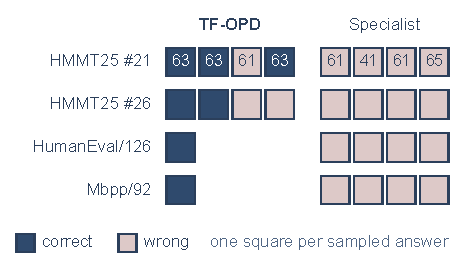
\includegraphics[width=0.5\textwidth]{figs/cases.pdf}
\caption{\textbf{Problems that \method solves and the specialist of the
domain does not.} One square per sampled answer: four per model on HMMT25,
and one for \method against four seeds of the coding specialist on the code
benchmarks. Numbers are the final answers given on HMMT25 problem~21, whose
reference answer is 63.}
\label{fig:cases-grid}
\end{figure}

\paragraph{HMMT25, problem 21.} \emph{In a two-dimensional cave with a
parallel floor and ceiling, two stalactites of lengths 16 and 36 hang
perpendicularly from the ceiling, while two stalagmites of heights 25 and 49
grow perpendicularly from the ground. If the tips of these four structures
form the vertices of a square in some order, compute the height of the
cave.} The answer is 63. The fused model answers 63 in three of its four
samples (Figures~\ref{fig:cases} and~\ref{fig:cases-grid}). It uses the fact
that the diagonals of a square share a midpoint: pairing the two stalactite
tips as one diagonal and the two stalagmite tips as the other, the midpoint
heights agree when $H-26=37$. The mathematics specialist is wrong in all four
samples. In the sample quoted in Figure~\ref{fig:cases}, it assumes a relation
between side lengths that leads to a contradiction, repeats one sentence about
``the correct configuration'', and ends with an unsupported answer.

\paragraph{HumanEval/126.} The task is to decide whether a list is sorted in
ascending order, returning false as well when a number occurs more than
twice. The fused model checks the order and then counts runs of equal
numbers, and passes the base and the additional tests. The coding specialist
mishandles the rule about repeated numbers in all four seeds and fails the
base tests.

\paragraph{Mbpp/92.} The task is to decide whether a number is undulating,
that is, whether two different digits alternate. The fused model requires
the first two digits to differ and every later digit to equal the digit two
places before it, and passes all tests. The coding specialist fails in all
four seeds: one tests for a palindrome and fails the base tests, and three
pass the base tests and fail the additional edge cases.
